% !TEX encoding = UTF-8 Unicode

\section{\large Hidden Markov Model}

%%%%%%%%%%%%%%%%%%%%

\subsection{Model Formulation}

\begin{frame}[fragile,t]{Model Formulation}
	\begin{figure}[!hbt]
    \center
    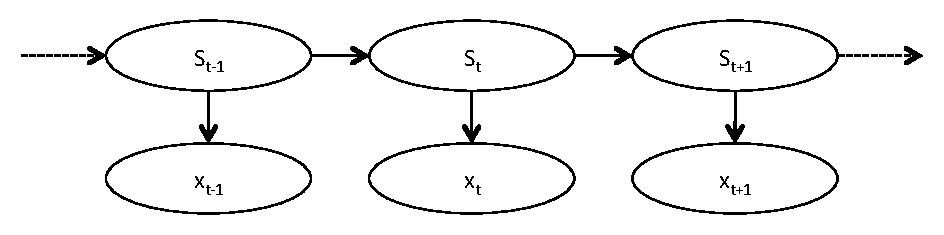
\includegraphics[width=0.65\textwidth]{HMM.pdf}
    \caption{Directed graph of a typical HMM}
    \label{fig:HMM:overview}
    \end{figure}

    \begin{itemize}
	\item A HMM is a \alert{doubly stochastic process}, explained with details in \cite{Zucchini:2009df}.
	\item The hidden states process $\{S_t \colon t = 1,2,\dots\}$ is a Markov chain:
		\[ \prob{S_t \mid \bS^{(t-1)}} = \prob{S_t \mid S_{t-1}},\ t = 2,3,\dots. \]
	\item The observed variable are conditionally distributed:
		\[ \prob{X_t \mid \bX^{(t-1)}, \bS^{(t-1)}} = \prob{X_t \mid S_t},\ t = 1,2,3,\dots. \]
	\end{itemize}
\end{frame}

%%%%%%%%%%%%%%%%%%%%

\subsection{Primary Statistics}

\begin{frame}[fragile,t]{Primary Statistics}
	\begin{itemize}
	\item State-dependent distribution (conditional distribution of $X$):
		\[ p_i(x) = \left \{ 
        \begin{array}{l l}
        \prob{X_t = x \mid S_t = i} & ,\text{if}\ X_t\ \text{is discrete,} \\
        f_t(x \mid S_t = i) & ,\text{if}\ X_t\ \text{is continuous.} \\
        \end{array} \right. \]
	\item Marginal distribution:
		\[ \prob{X_t = x} = \sum_{i=1}^{N} \prob{X_t = x \mid S_t = i}\prob{S_t = i} 
		= \sum_{i=1}^N p_i(x)\delta_i(t), \]
        or in form of matrix:
        \[ \begin{aligned}
		\prob{X_t = x} & = (\delta_1(t),\delta_2(t),\dots,\delta_N(t)) 
			\left ( \begin{array} {c c c}
				p_1(x) & & 0 \\
				& \ddots & \\
				0 & & p_N(x) \\
			\end{array} \right)
			\left ( \begin{array} {c}
				1 \\	\vdots \\	1 \\
			\end{array} \right) \\
		& = \bdelta(t)\bp(x)\one = \bpi\bGamma^{t-1}\bp(x)\one,
        \end{aligned} \]
    \end{itemize}
\end{frame}

\begin{frame}[fragile,t]{Primary Statistics}
    \begin{itemize}
    \item Likelihood:
		\[ L_T = \bpi\bp(x_1)\bGamma\bp(x_2)\bGamma\bp(x_3)\cdots\bGamma\bp(x_T)\one. \]
	\item Forward probabilities:
		\[ \begin{aligned}
		\balpha_t & = \bpi\bp(x_1)\bGamma\bp(x_2)\bGamma\bp(x_3)\cdots\bGamma\bp(x_t)
		= \bpi\bp(x_1)\prod_{s=2}^{t}\bGamma\bp(x_s),\\
		\alpha_t(j) & = \prob{\bX^{(t)} = \bx^{(t)}, S_t = j}.
		\end{aligned} \]
	\item Backward probabilities:
		\[ \begin{aligned}
		\bbeta_t & = \bGamma\bp(x_{t+1})\bGamma\bp(x_{t+2})\cdots\bGamma\bp(x_T)\one
		= \left(\prod_{s=t+1}^{T}\bGamma\bp(x_s)\right)\one, \\
		\beta_t(i) & = \prob{\bX^{(t+1:T)} = \bx^{(t+1:T)} \mid S_t = i},\ \prob{S_t = i}>0
		\end{aligned} \]
	\end{itemize}
\end{frame}

%%%%%%%%%%%%%%%%%%%%

\subsection{Expectation Maximization Algorithm}

\begin{frame}[fragile]{Expectation Maximization Algorithm}
	\begin{itemize}\vspace{0.4mm}
	\item Specifically known as Baum-Welch algorithm in the context of HMM,
		proposed separately in \cite{Baum:1966cy},\cite{Baum:1967gs} and \cite{Baum:1970do}.
	\item With forward and backward procedure, the algorithm has two steps:
		\begin{enumerate}
		\item \textbf{E step} calculates the expectations of (functions of) the missing data 
		conditional on the observations and the current estimate of $\btheta$;
		\item \textbf{M step} maximizes the CDLL w.r.t.\,$\btheta$.
		\end{enumerate}
	\item Essentially EM estimations are also a kind of \alert{MAP} estimation, 
		i.e.\,\alert{maximize a posterior} estimations.
	\end{itemize}
\end{frame}

\begin{frame}[fragile,t]{Expectation Maximization Algorithm}
	\begin{itemize}
	\item State value indicators:
		\[ u_j(t) = \left \{ \begin{array}{l l}
		1 & ,\text{iff}\ S_t = j \\
		0 & ,\text{otherwise}, \\
		\end{array} \right.
		\text{and}\ 
		v_{jk}(t) = \left \{ \begin{array}{l l}
		1 & ,\text{iff}\ S_{t-1} = j\ \text{and}\ S_t = k \\
		0 & ,\text{otherwise}. \\
		\end{array} \right. \]
	\item Maximize the complete-data log-likelihood (CDLL):
		\[ \begin{aligned}
		\log\left(\prob{\bx^{(T)},\bs^{(T)}}\right) & = 
		\underbrace{\sum_{j=1}^{N} u_j(1)\log\pi_j}_{\text{term 1}} + 
		\underbrace{\sum_{j=1}^{N}\sum_{k=1}^{N} 
			\left(\sum_{t=2}^Tv_{jk}(t)\right)\log\gamma_{jk}}_{\text{term 2}} \\ 
		& + \underbrace{\sum_{j=1}^{N}\sum_{t=1}^{T} u_j(t)\log p_j(x_t)}_{\text{term 3}}. 
		\end{aligned} \]
	\end{itemize}
\end{frame}

%%%%%%%%%%%%%%%%%%%%

\subsection{Prediction and Decoding}

\begin{frame}[fragile,t]{Prediction and Decoding}
	\begin{itemize}
	\item $h$-step forecast distribution:
		\[ \prob{X_{T+h} = x \mid \bX^{(T)} = \bx^{(T)}} = 
		\frac{\prob{\bX^{(T)} = \bx^{(T)}, X_{T+h} = x}}{\prob{\bX^{(T)} = \bx^{(T)}}} 
		= \frac{\balpha_T\bGamma^h\bp(x)\one}{\balpha_T\one}. \]
	\item Local decoding:
		\[ S_t^{\ast} = \argmax_{j = 1,2,\dots,N} \prob{S_t = j \mid \bX^{(T)} = \bx^{(T)}}. \]
	\item Global decoding:
		\[ \begin{aligned}
		\xi_{1i} & = \prob{S_1 = i,X_1 = x_1} = \pi_ip_i(x_1), \\
		\xi_{ti} & = \max_{s_1,s_2,\dots,s_{t-1}} 
			\prob{\bS^{(t-1)} = \bs^{(t-1)},S_t = i, \bX^{(T)} = \bx^{(T)}}, \\
		S_T & = \argmax_{i = 1,2,\dots,N} \xi_{Ti}, \\
		S_t & = \argmax_{i = 1,2,\dots,N} (\xi_{ti}\gamma_{i,S_{t+1}}).
		\end{aligned} \]
	\end{itemize}
\end{frame}
